\documentclass{beamer}

\usepackage{listings}
\usepackage{tabulary}
\usepackage{amsmath}
\usepackage[utf8]{inputenc}
\usetheme{Madrid}
\setbeamersize{text margin left=0.1\textwidth,text margin right=0.1\textwidth}
\setbeamertemplate{section in toc}{\inserttocsection}
\lstset{language=python,
        keywordstyle=\color{red},
        basicstyle=\ttfamily,
        basicstyle=\small,
        frame = single,
        framexleftmargin=15pt,
        numbers=left,
        numberstyle=\small,
        numbersep=5pt,
        xleftmargin=0.05\textwidth,
        columns=fullflexible}
\definecolor{dgreen}{rgb}{0.,0.6,0.}
\definecolor{goldenrod}{rgb}{.9,0.6,0.1}

%Information to be included in the title page:
\title{Non-Negative Matrix Factorization}
\subtitle{Interpretable Topic Modeling}
\author{Cary Goltermann}
\institute{Galvanize}
\date{2016}

\AtBeginSubsection[]
{
  \begin{frame}
    \frametitle{Overview}
    \tableofcontents[currentsection,currentsubsection]
  \end{frame}
}

\begin{document}

\frame{\titlepage}

\begin{frame}
  \frametitle{Overview}
  \tableofcontents[]
\end{frame}

\section{Topic Modeling}
\subsection{Motivation}
\begin{frame}
  \frametitle{Thinking About Topic Modeling}
  As a form of unsupervised learning, topic modeling attempts to extract an underlying structure from our data. \vspace{4mm}

  Specifically, we will endeavor to discover an underlying set of ``topics'' that describe high level ideas about our data well.
\end{frame}

\subsection{Thinking About Topics}
\begin{frame}
  \frametitle{Thinking About Topics}
  Consider having the term-frequency matrix for a corpus of documents, all coming from some sort of related source; articles from a newspaper possibly? \vspace{4mm}

  In trying to discover topics, or latent features, in these data, we might expect to find such overarching ones as: Sports, International, Arts and Leisure, etc.
\end{frame}

\subsection{Assumptions}
\begin{frame}
  \frametitle{Topic Analysis Assumptions}
  \begin{enumerate}
    \item The observations are well described by underlying topics. E.g. All sports articles will have similar sportsy words. In math, each topic has a corresponding distribution of words:
      $$ tf(word | topic) $$ \vspace{-6mm} \pause
    \item The words in a document can be represented by an appropriate combination of topics. E.g. An article about FIFA could be represented by the topics International and Sports. Math:
      $$ tf(word | doc) = \sum_{t \in T} tf(word | topic) \times w(t | doc) $$
      Where $T$ is the set of topics and $w$ is some positive weight.
  \end{enumerate}
\end{frame}

\section{Non-Negative Matrix Factorization}
\subsection{The Math}
\begin{frame}
  \frametitle{NMFactorization}
  Another way to mathematically express the topic modeling assumptions is through the equation: \vspace{6mm}

  \begin{center}
    {\LARGE $ X \approx W \cdot H $},  $ \qquad w_{i, j}\: \& \: h_{i, j} \geq 0 $ \vspace{4mm}
  \end{center}

  Or, X can be approximated by the dot product of two matrices. Hence factorization.
\end{frame}

\begin{frame}
  \frametitle{Thinking in Dimensions}
  How can we think about the values in each of these matrices, $W$ and $H$. Let's look at their dimensions!

  {\LARGE $$ \underset{\small n\: x \: m}{X} \approx \underset{\small n\: x \: k}{W} \cdot \underset{\small k\: x \: m}{H} $$} \vspace{4mm}

  We can easily rationalize that when the internal dimension, $k$, is $\geq m$ we can perfectly recreate $X$. \vspace{6mm} \pause

  \centering
  \textcolor{blue}{So what happens when this dimension, $k$, is smaller than $m$?}
\end{frame}

\begin{frame}
  \frametitle{A Smaller Number of Decomposed Dimensions}
  \begin{itemize}
    \item In looking at the dimensions of the $W$ matrix from our decomposition, we notice that the number of rows remains the same, as we would expect. \vspace{4mm}

    \item Thus, the rows of $W$ must represent some information about each row in $X$. \vspace{4mm}

    \item When we use a smaller number of dimensions to represent our data in W, a.k.a $k < m$, we will necessarily find that some sort of data compression is happening. \vspace{4mm}

    \item Or, in math, we are projecting our data onto a lower dimensioned basis.
  \end{itemize}
\end{frame}

\subsection{Latent Features}
\begin{frame}
  \frametitle{Topics as Latent Feature Bases}
  It, somewhat magically, turns out that when we conduct a factorization of this nature each of bases in the lower dimensional representation of $X$, a.k.a. $W$, can be viewed of as a latent feature. \vspace{4mm}

  These latent features are discovered as somewhat of a side-effect of projecting into a smaller number of dimensions, of performing some sort of compression. \vspace{2mm}

  \begin{block}{The Latent Features are Topics}
    The values of the each row in the latent feature space correspond to their strength with the associated topic.
  \end{block}
\end{frame}

\begin{frame}
  \frametitle{Example $W$ Matrix}
  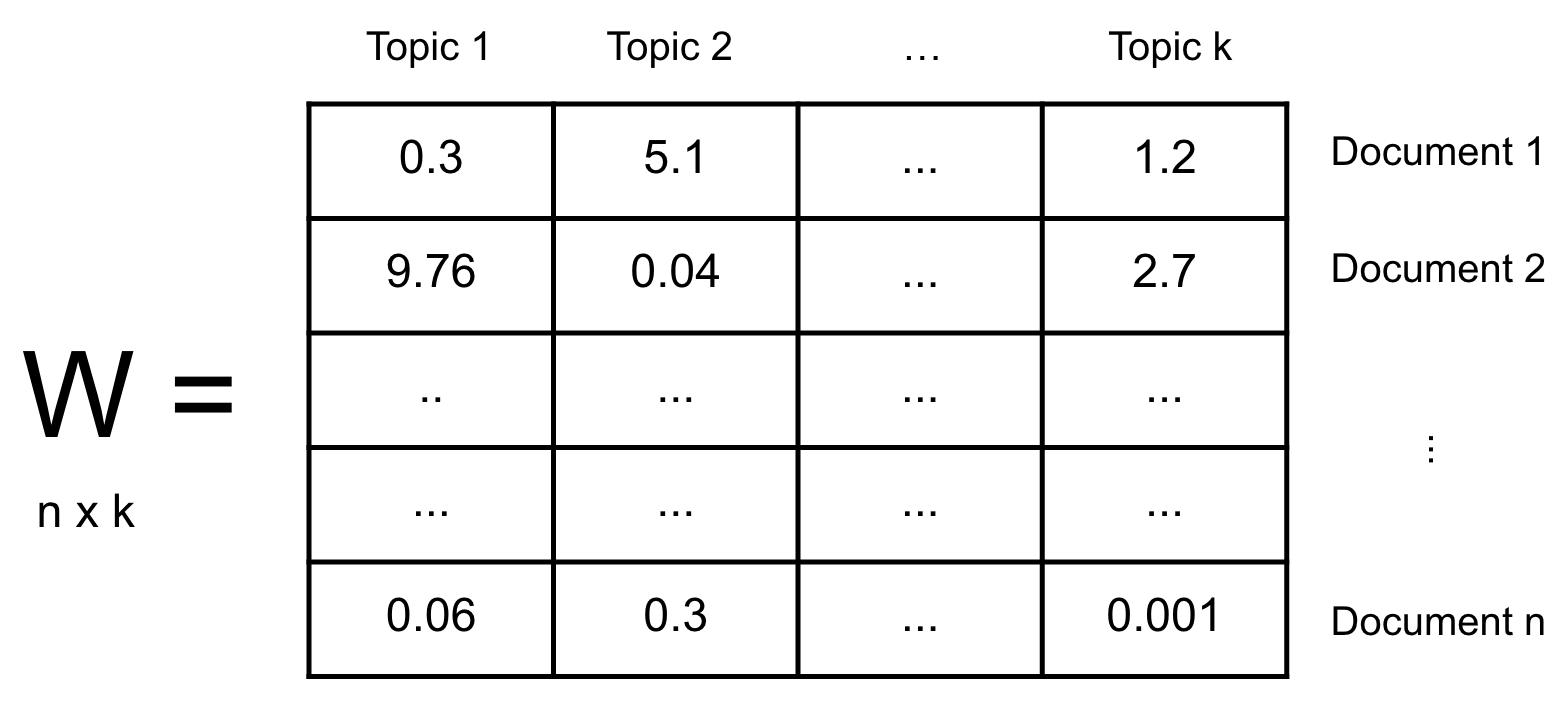
\includegraphics[width=\textwidth]{images/w_matrix.png}
\end{frame}

\subsection{Interpretation}
\begin{frame}
  \frametitle{Identifying Topics}
  How, then, do we figure out what topics these latent feature bases correspond to? Consider that this is an unsupervised approach, so it's not like we're telling it to look for sports words. \vspace{0.5mm}

  To put ``labels'' on our latent features and identify them as topics we can do one of to things. \vspace{2mm} \pause

  \begin{enumerate}
    \item Look at the observations that load heavily on each topic and manually inspect them, trying to identify some commonalities, a.k.a. the latent features. \vspace{2mm} \pause
    \item Inspect the $H$ matrix and see what features contribute to each topic.
  \end{enumerate} \vspace{2mm} \pause
\end{frame}

\begin{frame}
  \frametitle{Inspecting the $H$ Matrix}

  How would we inspect the $H$ matrix, and why would doing so make sense? \pause \textcolor{blue}{Again, let's look at the dimensions!}

  {\large $$ \underset{\small n\: x \: m}{X} \approx \underset{\small n\: x \: k}{W} \cdot \underset{\small k\: x \: m}{H} $$} \vspace{-3mm}

  \begin{itemize}
    \item We see that the number of columns in $X$, $m$, is the same as in $H$.
    \item From this we can reason that the columns in $H$ represent some information about the columns in $X$.
    \item More specifically, we can view the features in $X$ as being the basis for our latent topics.
  \end{itemize}
\end{frame}

\begin{frame}
  \frametitle{Example $H$ Matrix}
  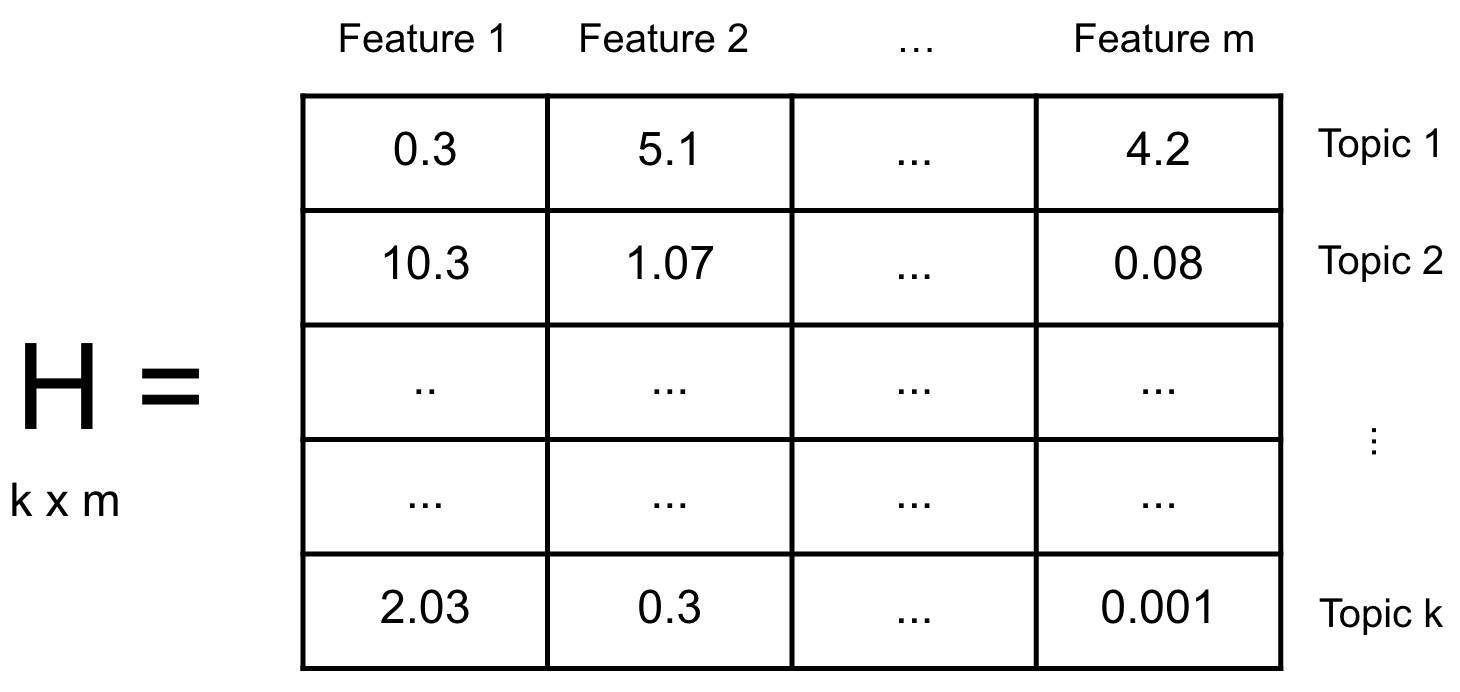
\includegraphics[width=\textwidth]{images/h_matrix.png}
\end{frame}

\begin{frame}
  \frametitle{Example $H$ Matrix}
  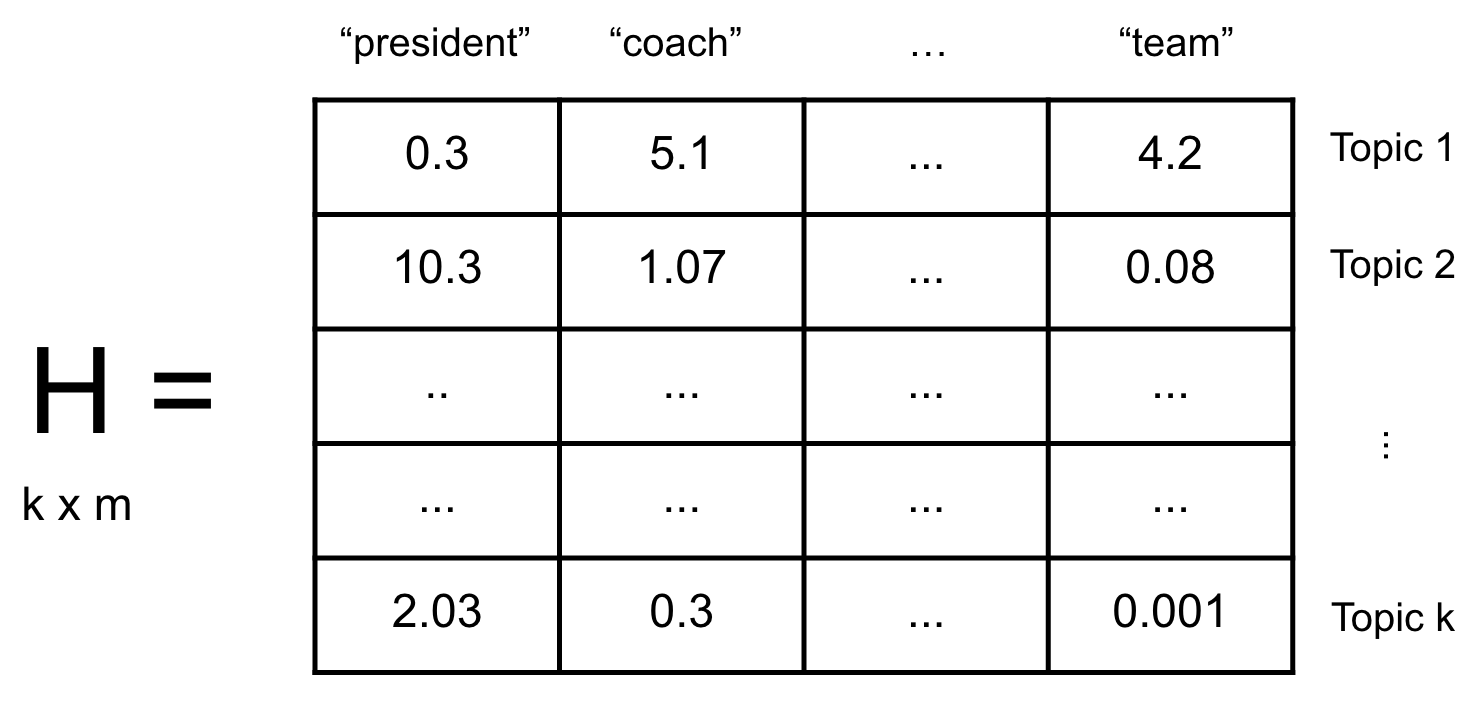
\includegraphics[width=\textwidth]{images/h_topics.png} \vspace{2mm} \pause

  \centering
  Topic 1 $ \rightarrow $ Sports?

  Topic 2 $ \rightarrow $ Politics??
\end{frame}

\begin{frame}
  \frametitle{Choosing $k$}
  Unfortunately, choosing $k$ is more of an art than a science. We can look at how ``good'' of an approximation $WH$ is for $X$ and try to find the smallest $k$ that makes it suitably small. \vspace{4mm}

  At the end of the day, though, $k$, is likely going to be chosen based on intuition that you derive from inspecting the topics and possibly from some domain knowledge.
\end{frame}

\begin{frame}
  \frametitle{Reflection}
    \textbf{\textcolor{blue}{Time}}: 2 minutes \vspace{4mm}

    \textbf{\textcolor{blue}{Exercise}}: Discuss, in groups of 2-3, how we can think about the rows in $W$ and the columns in $H$.
\end{frame}

\begin{frame}
  \frametitle{Thinking About Matrix Factorizations}
  We have already explored two other factorization techniques, PCA and SVD. What's the difference between those and NMF? \vspace{4mm} \pause

  Apart from the obvious that PCA and SVD decompose into three matrices and NMF only two; the main difference is the non-negativity constraint. \vspace{6mm}

  \begin{columns}
    \column{0.8\textwidth}
    \textit{Note: the other, oft-forgotten difference is that the bases in NMF are not orthogonal like in PCA/SVD.}
  \end{columns}
\end{frame}

\begin{frame}
  \frametitle{Why All the Non-Negativity?}
  Why do we care about having all the entries in the factorized matrices be positive? \vspace{5mm} \pause

  It comes down to the interpretability of the topics. Remember, in PCA/SVD we were allowed negative entries in our matrices. \vspace{5mm} \pause

  However, when looking at our data, we frequently find that we have all positive entries in $X$. So, when it comes to interpreting the negative values in the decomposed matrices, how do we think about them?
\end{frame}

\begin{frame}
  \frametitle{Comparing PCA/SVD and NMF}
  \begin{columns}
    \column{1.1\textwidth}
    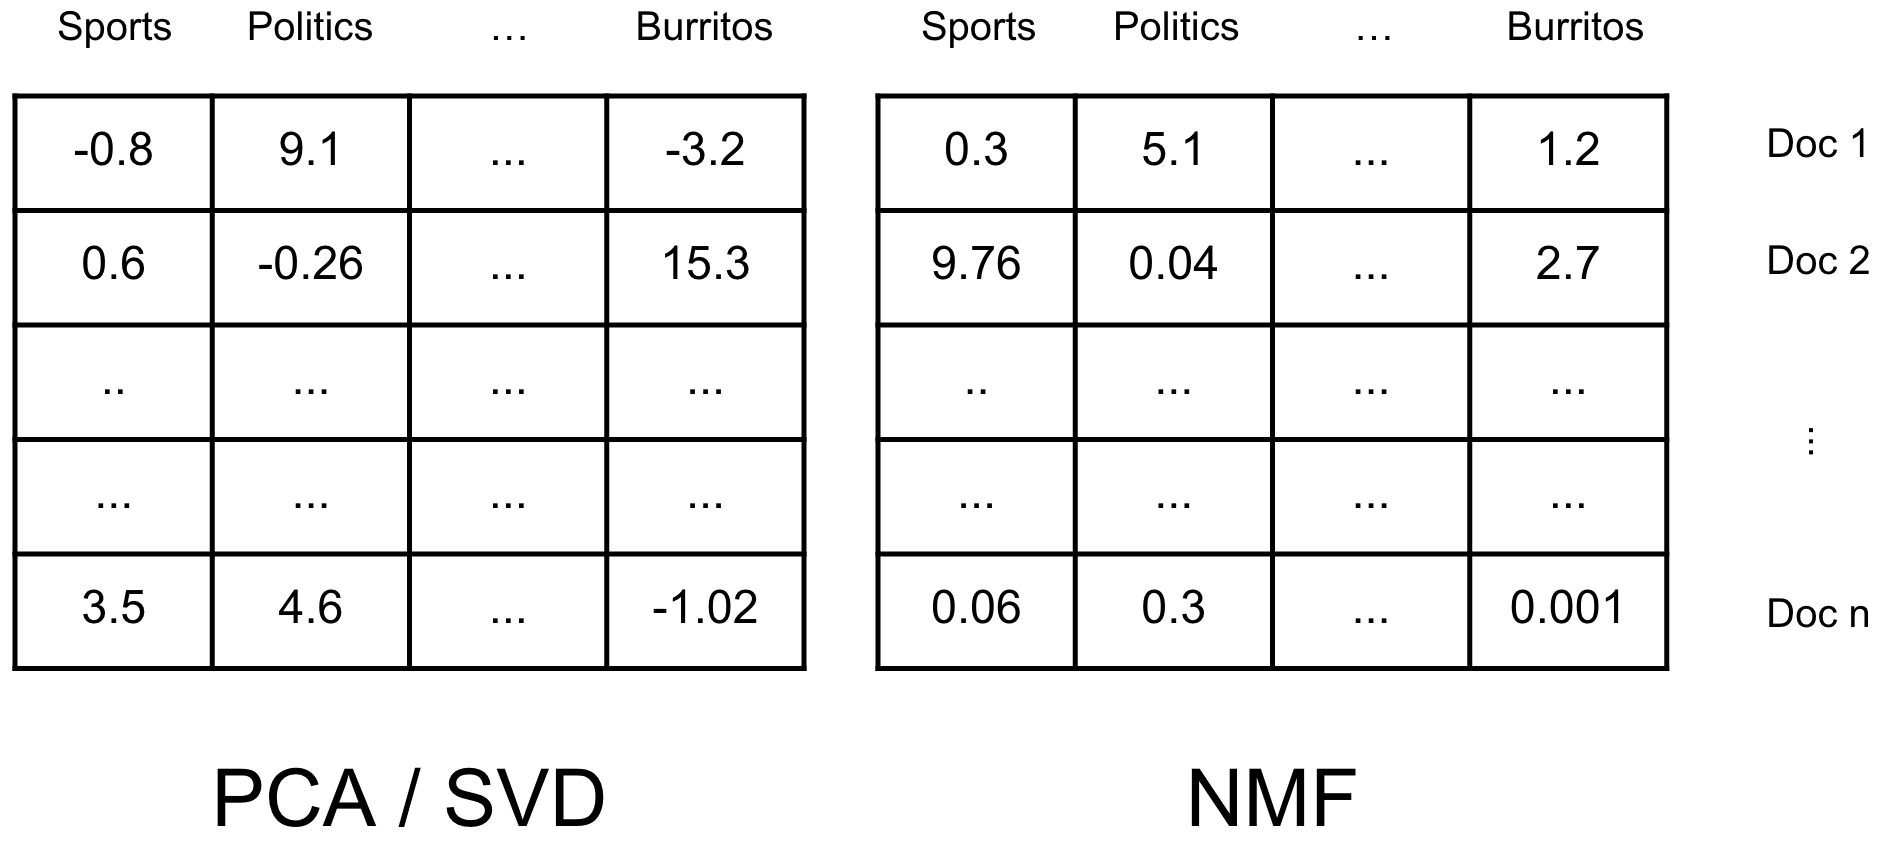
\includegraphics[width=\textwidth]{images/pca_nmf.png}
  \end{columns} \vspace{4mm}

  Have only additive components of a topic makes more sense!
\end{frame}

\begin{frame}
  \frametitle{Reconstructing X}
  X is approximated by the inner product of $W$ and $H$. \vspace{4mm}
  \begin{columns}
    \column{1.1\textwidth}
    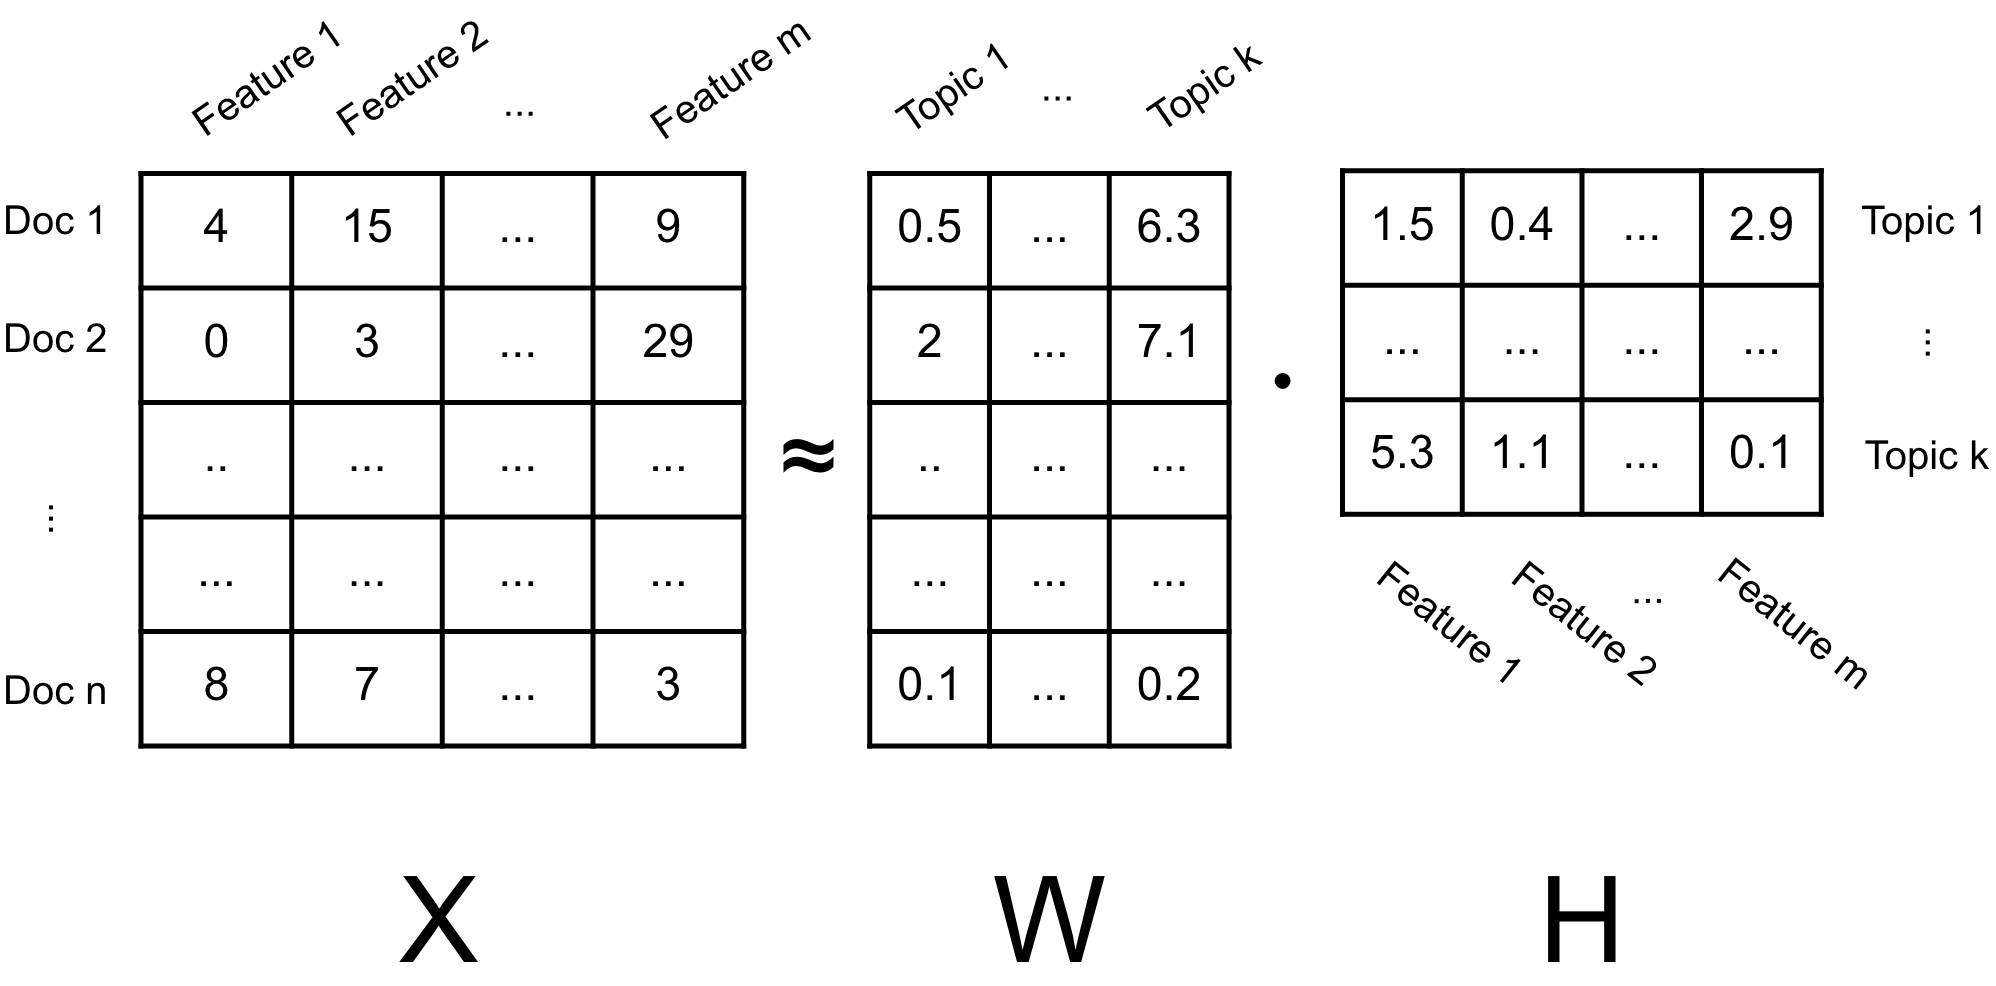
\includegraphics[width=\textwidth]{images/x_w_h.png}
  \end{columns} \vspace{4mm}
\end{frame}

\begin{frame}
  \frametitle{Reconstructing X}
  How do we reconstruct only one cell of $X$? \vspace{4mm}
  \begin{columns}
    \column{1.1\textwidth}
    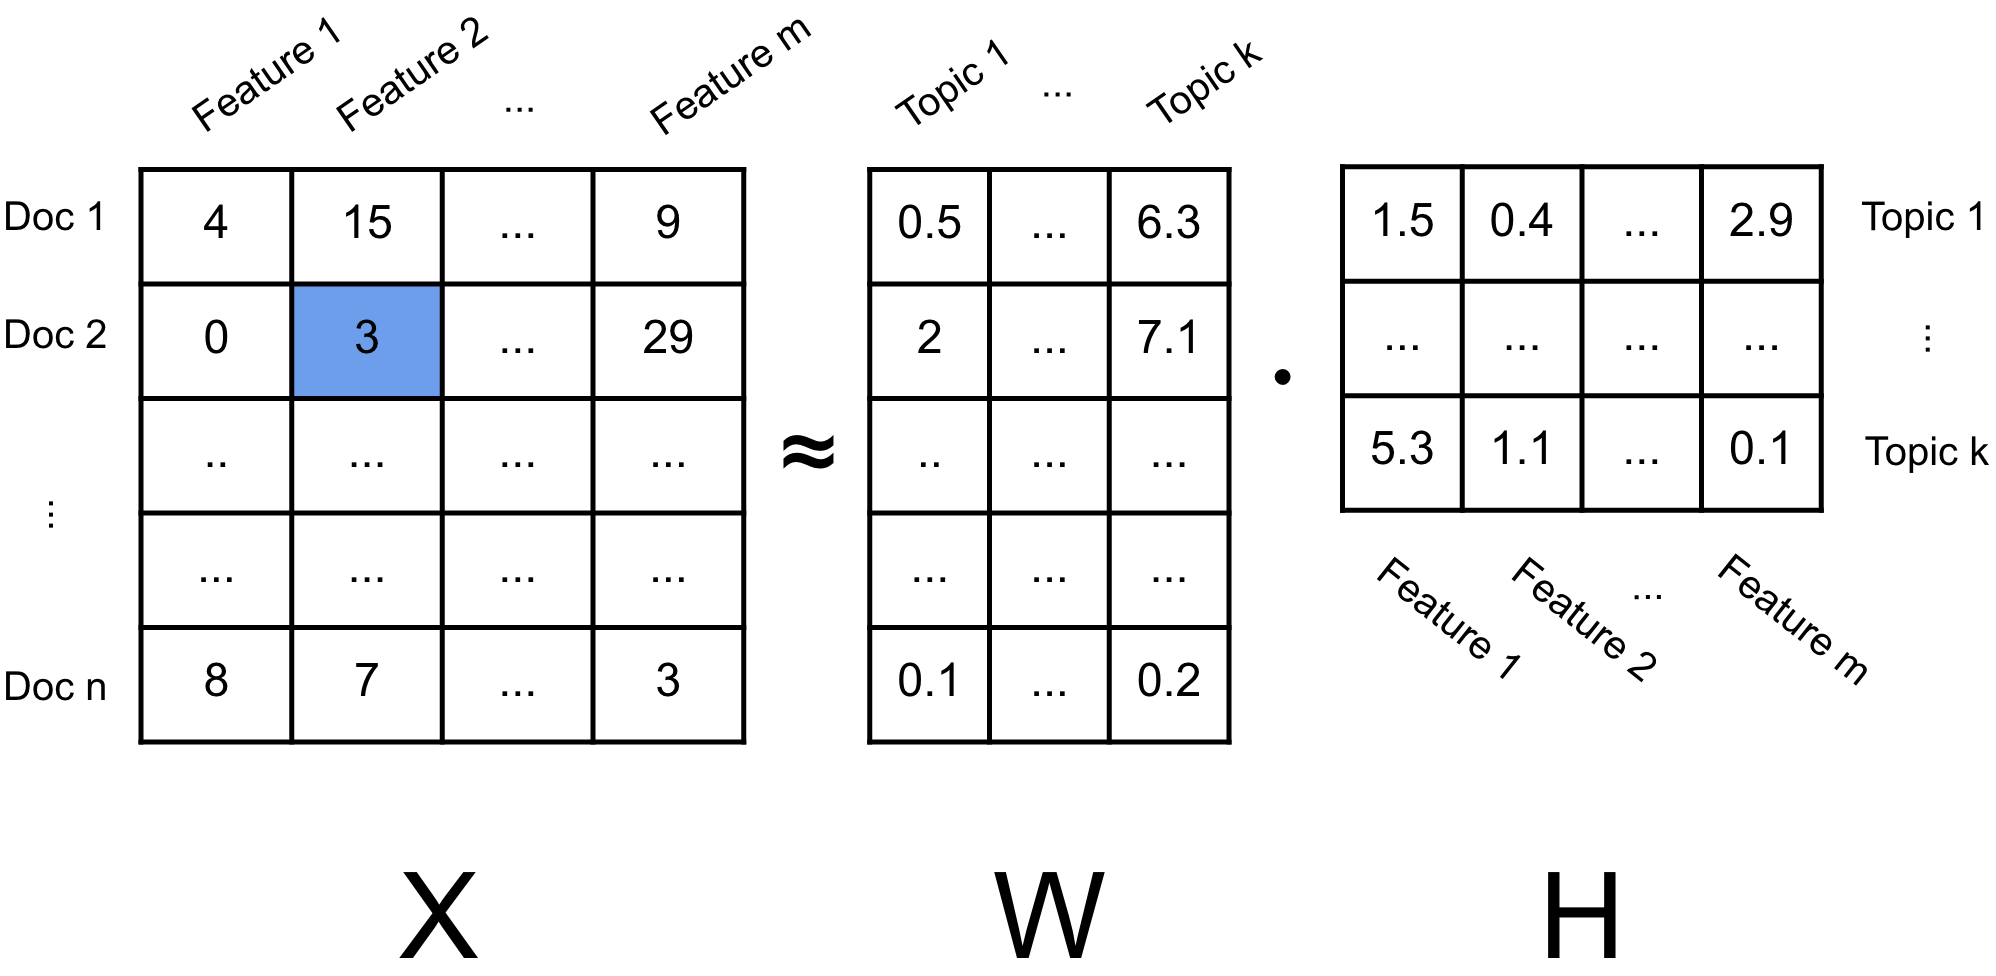
\includegraphics[width=\textwidth]{images/x_w_h_cell.png}
  \end{columns} \vspace{4mm}
\end{frame}

\begin{frame}
  \frametitle{Reconstructing X}
  Inner product of $W$ and $H$'s correct column and row. \vspace{4mm}
  \begin{columns}
    \column{1.1\textwidth}
    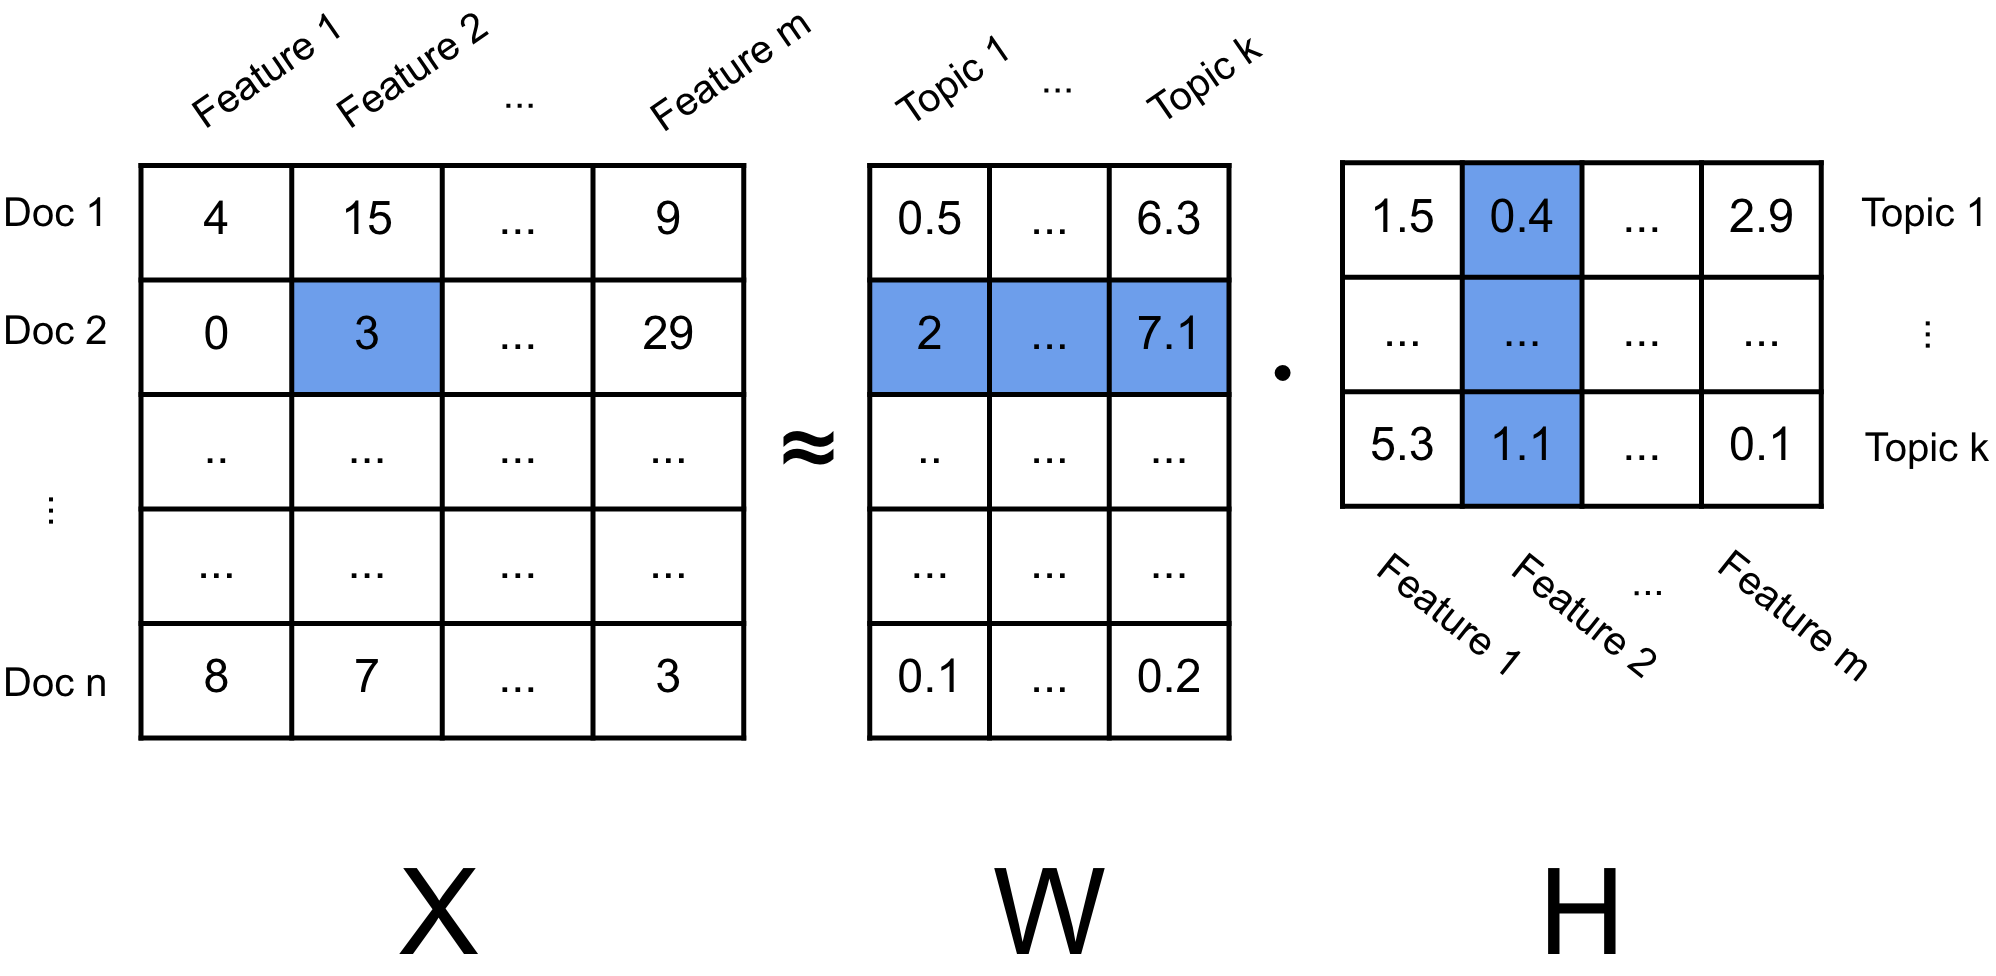
\includegraphics[width=\textwidth]{images/x_w_h_reconstruction.png}
  \end{columns} \vspace{4mm}
\end{frame}

\begin{frame}
  \frametitle{How Could We Find Such Matrices?}
  So, we're trying to find matrices, $W$ and $H$ such that:
  $$ X \approx W \cdot H  \qquad w_{i, j}\: \& \: h_{i, j} \geq 0 $$
  With PCA and SVD we have a closed form solution for finding the those factorizations. Unfortunately, we don't have such a solution for NMF. \vspace{6mm} \pause

  \centering
  \textcolor{blue}{So how do we find $W$ and $H$?}
\end{frame}

\subsection{Algorithms}
\begin{frame}
  \frametitle{Finding $W$ and $H$}
  We call this type of optimization problem biconvex, it's convex in either $W$ \textbf{or} $H$ but not both, and there's a straightforward way we can brute force an approximate solution in this case. \vspace{4mm} \pause

  We can notice, that, while there is no closed form solution for $W$ \textbf{and} $H$, if we hold one of these matrices constant there \textbf{is} a closed form optimum for the other. \vspace{4mm}

  This leads us to the  \textbf{\textcolor{blue}{Alternating Least Squares}} algorithm.
\end{frame}

\begin{frame}
  \frametitle{Alternating Least Squares (ALS)}
  We will take advantage of the biconvexivity by alternating which matrix, $W$ or $H$, that we treat as stationary, solving for the other's optimal values, and then clipping all the negative values in that solution to 0. \vspace{4mm} \pause

  Pseudo-code:
  \begin{enumerate}
    \item Initialize W to small, positive, random values.
    \item For max number of iterations:
      \begin{enumerate}
        \item Find the least squares solution to $ X = W \cdot H $ w.r.t. $H$.
        \item Clip negative values in H to 0: $ H < 0 = 0$.
        \item Find the least squares solution to $ X = W \cdot H $ w.r.t. $W$.
        \item Clip negative values in H to 0: $ W < 0 = 0$.
      \end{enumerate}
  \end{enumerate}
\end{frame}

\begin{frame}
  \frametitle{ALS Pros and Cons}
  \begin{columns}
    \column{0.5\textwidth}
    \begin{center} {\LARGE \textcolor{blue}{Pros}} \end{center}
    \column{0.5\textwidth}
    \begin{center} {\LARGE \textcolor{blue}{Cons}} \end{center}
  \end{columns} \vspace{4mm}
  \begin{columns}
    \column[T]{0.5\textwidth}
    \begin{itemize}
      \item Fast
      \item Works well in practice
    \end{itemize}
    \column[T]{0.5\textwidth}
    \begin{itemize}
      \item Non-negativity enforced in an ad hoc way
      \item Not guaranteed to find a local minimum much less global
      \item No convergence theory
    \end{itemize}
  \end{columns}
\end{frame}

\begin{frame}
  \frametitle{Cost Function}
  Another way that we could solve this optimization problem is with gradient descent. What do we need in order to descend a gradient, though? \vspace{4mm} \pause

  A \textcolor{blue}{cost function}! What should our cost function for this optimization problem be? \vspace{4mm} \pause

  First we're going to define how much we're missing in our approximation of $X$, the matrix $X - WH$ as the reconstruction error. \vspace{4mm} \pause

  Then, we're going to use the generalization of euclidean distance on matrices, also known as the Frobenius norm on the reconstruction error to quantify how well we are approximating $X$.
\end{frame}

\begin{frame}
  \frametitle{Gradient Descent}
  Let the Frobenius norm of the reconstruction error be the quantity that we are trying to minimize:

  $$ \underset{W, H}{min} \; \big\Vert X - W H \big\Vert^2_{F} $$ \vspace{0.5mm}

  From this, with a little be of matrix calculus we can determine that the update rules for a single entry in $W$ and $H$ are: \vspace{-1mm}

  \begin{align*}
    H_{a, \mu} &\leftarrow H_{a, \mu} + \nu_{a, \mu}\big[(W^T X)_{a, \mu} - (W^T WH)_{a, \mu}\big] \\
    W_{i, a} &\leftarrow W_{i, a} + \nu_{i, a}\big[(XH^T)_{i, a} - (WHH^T)_{i, a}\big]
  \end{align*}
\end{frame}

\begin{frame}
  \frametitle{Are You Sure About that Calculus?}
  \begin{columns}
    \column{0.55\textwidth}
    
\includegraphics[width=\textwidth]{images/newton_meme.png}
  \end{columns}
\end{frame}

\begin{frame}
  \frametitle{Multiplicative Update Rules}
  If we are clever about the value that we choose as our step size, $\nu$ we can reduce those gradient descent updates to what are known as the multiplicative update rules. \vspace{2mm}
  Let: \vspace{1mm}

  \begin{columns}
    \column{0.5\textwidth}
      $$ \nu_{a, \mu} = \frac{H_{a, \mu}}{(W^T WH)_{a, \mu}} $$
    \column{0.5\textwidth}
      $$ \nu_{i, a} = \frac{W_{i, a}}{(WHH^T)_{i, a}} $$
  \end{columns} \vspace{4mm}

  Then we can rewrite the gradient descent updates as: \vspace{0.5mm}

  \begin{columns}
    \column{0.5\textwidth}
      $$ H_{a, \mu} \leftarrow H_{a, \mu} \frac{(W^T X)_{a, \mu}}{(W^T WH)_{a, \mu}} $$
    \column{0.5\textwidth}
      $$ W_{i, a} \leftarrow W_{i, a} \frac{(XH^T)_{i, a}}{(WHH^T)_{i, a}} $$
  \end{columns} \vspace{4mm}

  These updates will be iteratively performed from $W$ and $H$ initialized with random, small, positive values.
\end{frame}

\begin{frame}
  \frametitle{Lack of Unique Solution}
  It's important to know that NMF, as a topic modeling algorithm will almost \textcolor{blue}{never yield a unique solution} due to the non-negativity constraint we're putting on the entries in $W$ and $H$. \vspace{4mm}

  The ramifications of this are that the latent topics that you discover each time you run NMF can change quite a lot. This is somewhat unsatisfying, however, it's the price we pay for interpretable topics.
\end{frame}

\begin{frame}
  \frametitle{Transforming New Data}
  Once we have a factorization set up we might want to be able to project a new document into our latent feature space. How would we do this? \vspace{4mm} \pause

  It's actually not particularly difficult. We can use the same OLS technique we learned in linear regression. Let's see how this works. \vspace{4mm}
\end{frame}

\begin{frame}
  \frametitle{OLS for Transforming New Data}
  What we have is a new row in our $X$ matrix, $X_{new}$ and we're trying to find a representation in the space spanned by the columns of $W$, a.k.a. $W_{new}$. So what we're actually trying to solve is the equation:

  $$ \underset{\small 1\: x \: m}{X_{new}} = \underset{\small 1\: x \: k}{W_{new}} \cdot \underset{\small k\: x \: m}{H_{same}} $$

  for $W_{new}$.

  \noindent\hfil\rule{\textwidth}{.4pt}\hfil \vspace{1mm}

  Looks a lot like:
  $$ \underset{\small n\: x \: 1}{y} = \underset{\small n\: x \: m \: m\: x \: 1}{X \quad \beta} $$

  But it's worth noting that this functionality is available to you built into existing NMF algorithms, e.g. sklearn's (with the $transform()$ method).
\end{frame}

\begin{frame}
  \frametitle{Side Notes}
  NMF is considered a soft clustering, so called because each of the latent features can be viewed as a cluster, and because each observation can be partially in more than one "cluster". \vspace{4mm}

  There are a number of penalties that have been devised to make the factorizations more friendly to interpretation. \vspace{2mm}

  \begin{description}
    \item[Simple] Ridge / Lasso regularization.
    \item[Complex] Try to enforce sparsity in $W$ and $H$.
  \end{description}
\end{frame}
\end{document}
